%===============================================================================
% PROPERTIES
%===============================================================================
% $Id$
%===============================================================================


%===============================================================================
% Configuration
%===============================================================================


%-------------------------------------------------------------------------------
% \documentclass and \usepackage directives
%-------------------------------------------------------------------------------
\documentclass[a4paper,fleqn,titlepage]{article}
%\usepackage{ngerman}
\usepackage[latin1]{inputenc}
\usepackage[T1]{fontenc}
\usepackage[small,hang,bf]{caption2}
\usepackage{fancyhdr}
\usepackage[nice]{nicefrac}
\usepackage{color,listings}
\usepackage{alltt}


% Compilation with latex or pdflatex?
\newif\ifpdf 
\ifx\pdfoutput\undefined 
  \pdffalse
\else
  \pdfoutput=1 
  \pdftrue 
\fi 

% Compilation with pdflatex
\ifpdf
 
  \usepackage[pdftex]{graphicx}

  \usepackage[
    pdftex,
    a4paper,
    bookmarks,
    pdfstartview=FitH,    % starts with page width
    bookmarksopen,        % opens index
    bookmarksnumbered,    % index with numbering
    colorlinks,           % links with color, otherwise with border
    linkcolor=blue,       % Standard red
    citecolor=blue,       % Standard green
    urlcolor=magenta,     % Standard cyan
    filecolor=blue
  ]{hyperref} 

  \pdfinfo{
    /Title      (PROPERTIES)
    /Author     (Thomas Weibel)
    /Subject    (Eiffel programming)
    /Keywords   (Programming, Eiffel, Configuration)
  }

  % Use default Acrobat reader fonts
  \usepackage{mathpazo}

  % Use CM fonts (increases document size)
  % \usepackage{ae}

% Compilation with latex
\else 

  \usepackage{graphicx} 

\fi


%-------------------------------------------------------------------------------
% Configure \maketitle
%-------------------------------------------------------------------------------
\title{EiffelRSS \\ PROPERTIES \\ Developer Guide}
\author{
  Michael K\"aser <kaeserm@student.ethz.ch>
  \and 
  Martin Luder <luderm@student.ethz.ch>
  \and 
  Thomas Weibel <weibelt@student.ethz.ch>
}
\date{\today}


%-------------------------------------------------------------------------------
% Configure fancyhdr
%-------------------------------------------------------------------------------
\pagestyle{fancy}

\renewcommand{\headrulewidth}{0.1 pt}
\renewcommand{\footrulewidth}{0.1 pt}

\fancypagestyle{plain}{
  \lhead{\nouppercase{\leftmark}}
  \chead{}
  \rhead{\thepage}
  \lfoot{PROPERTIES}
  \cfoot{}
  \rfoot{Developer Guide}
}

\lhead{\nouppercase{\leftmark}}
\chead{}
\rhead{\thepage}

\lfoot{PROPERTIES}
\cfoot{}
\rfoot{Developer Guide}


%-------------------------------------------------------------------------------
% Configure listings
%-------------------------------------------------------------------------------
\lstset{showstringspaces=false,
  breaklines=true,
  breakindent=0pt,
  prebreak=\mbox{\tiny$\searrow$},
  postbreak=\mbox{{\color{blue}\tiny$\rightarrow$}},
  frame=trBL,
  framerule=0.75pt,
  framesep=4pt,
  rulesep=0.75pt  
}


%-------------------------------------------------------------------------------
% Common configuration
%-------------------------------------------------------------------------------
\setlength{\parindent}{0em}
\setlength{\parskip}{1.5ex plus0.5ex minus0.5ex}
\sloppy
\setlength{\mathindent}{0em}


%-------------------------------------------------------------------------------
% Commandos
%-------------------------------------------------------------------------------
\newcommand{\hr}{\rule{\textwidth}{1pt}}


%===============================================================================
% Document
%===============================================================================
\begin{document}

\begin{titlepage}
  \newlength{\centeroffset}
  \setlength{\centeroffset}{-0.5\oddsidemargin}
  \addtolength{\centeroffset}{0.5\evensidemargin}

  \thispagestyle{empty}

  \noindent
\includegraphics[width=\textwidth]{../../figures/big_ETH}\\[-3mm]
  \hr

  \vspace*{\stretch{1}}

  \makebox[0pt][l]{
    \begin{minipage}{\textwidth}
      \flushright{
        \Huge\bfseries EiffelRSS
      }

      \noindent\rule{\textwidth}{3pt}\\[2.5ex]

      \hfill\emph{
        \Large PROPERTIES: Developer Guide
      }
    \end{minipage}
  }

  \vspace{\stretch{1}}

  \makebox[0pt][l]{
    \begin{minipage}{\textwidth}
      \flushright{
        \bfseries 
        Michael K\"aser <kaeserm@student.ethz.ch>\\[0.3ex]
        Martin Luder <luderm@student.ethz.ch>\\[0.3ex]
        Thomas Weibel <weibelt@student.ethz.ch>\\[0.3ex]
      }
    \end{minipage}
  }

  \vspace{\stretch{1}}

  \noindent\hr\\[1mm]
  
\includegraphics[width=\textwidth]{../../figures/big_inf}
\end{titlepage}

% Use roman page numbering
\pagenumbering{roman}

\begin{abstract}
  \texttt{PROPERTIES} represents a persistent set of properties. The
  properties can be saved to a file or loaded from a file.
\end{abstract}

\clearpage
\tableofcontents

\clearpage
\listoffigures

\newpage

\section{Overview}
\label{sec:overview}

% Set page counter to zero
\setcounter{page}{0} 

% Use arabic page numbering
\pagenumbering{arabic}

\texttt{PROPERTIES} represents a persistent set of properties. The
properties can be saved to a file or loaded from a file.

Each key and its corresponding value in the property list is a string.

A property list can contain another property list as its default. This
default property list is searched if the property key is not found in
the original property list.

\texttt{PROPERTIES} is similar to the \texttt{java.util.Properties}
class. The main difference is, that \texttt{PROPERTIES} doesn't
support keys and values separated by whitespace only. It always
expects \texttt{:} or \texttt{=} as a separator between key and value.

See figure \ref{fig:cluster} for an overview of the cluster.

\begin{figure}[htbp]
  \centering
  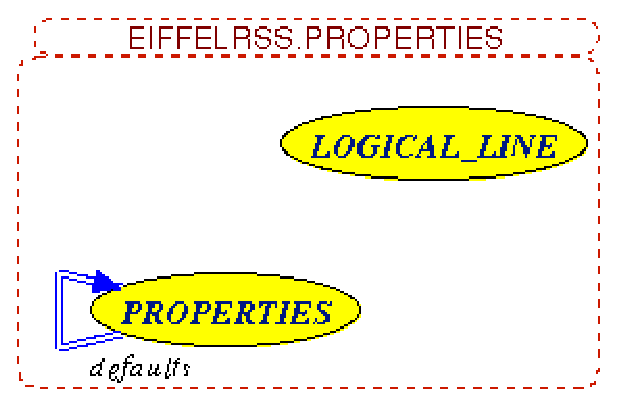
\includegraphics[scale=.6]{./figures/EIFFELRSS_PROPERTIES}
  \caption{BON diagram of cluster \texttt{PROPERTIES}}
  \label{fig:cluster}
\end{figure}

Figure \ref{fig:classes} shows the classes \texttt{PROPERTIES} and
\texttt{LOGICAL\_LINE}.

\begin{figure}[htbp]
  \centering
  
\includegraphics[scale=.6]{./figures/PROPERTIES}
  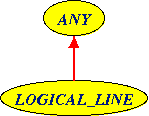
\includegraphics[scale=.6]{./figures/LOGICAL_LINE}
  \caption{BON diagram of classes \texttt{PROPERTIES} and \texttt{LOGICAL\_LINE}}
  \label{fig:classes}
\end{figure}

\newpage

\section{Usage}
\label{sec:usage}

\begin{lstlisting}[language=Eiffel]
class USAGE_EXAMPLE

create 
  make

feature -- Initialization

  make is
      -- Creation procedure.
    do                  
      -- Open files
      create output_file.make_create_read_write ("settings.txt")
                        
      -- Create properties
      create settings.make (10)
      create settings_new.make (10)
                        
      -- Create, display, store and load settings
      -- Put some values
      settings.put ("Benjy, Frankie", "mice")
      settings.put ("Slartibartfast", "fjord designer")
      -- Display properties
      io.put_string (settings.list)
      -- Store properties
      io.put_string ("%NSaving properties%N")
      settings.store (output_file, "PROPERTIES test")
      -- Load properties
      io.put_string ("Loading properties%N%N")
      settings_new.load (output_file)
      -- Display properties
      io.put_string (settings_new.list)
    end
                
feature -- Arguments

  settings, settings_new: PROPERTIES
      -- Properties
                        
  output_file: PLAIN_TEXT_FILE
      -- Files for input, output and the defaults
        
end -- class USAGE_EXAMPLE
\end{lstlisting}


\section{Features}
\label{sec:features}

Because \texttt{PROPERTIES} inherits from \texttt{HASH\_TABLE [STRING,
  STRING]}, all features of \texttt{HASH\_TABLE} can be applied to a
\texttt{PROPERTIES} object, e.g. \texttt{put}, \texttt{has},
\texttt{replace} etc.


\subsection{Initialization}
\label{sec:initialization}


\subsubsection{make}

\begin{lstlisting}[language=Eiffel]
make (n: INTEGER)
  -- Create an empty property table of initial size `n'
\end{lstlisting}


\subsubsection{make\_defaults}

\begin{lstlisting}[language=Eiffel]
make_defaults (n: INTEGER; def: PROPERTIES)
  -- Create a property table with `d' as default values and initial size `n'
\end{lstlisting}


\subsection{Access}
\label{sec:access}


\subsubsection{get}

\begin{lstlisting}[language=Eiffel]
get (key: STRING): STRING
  -- Item associated with `key', if present
  -- otherwise default value from `defaults'
\end{lstlisting}

Searches for the property with the specified key in this property
list. If the key is not found, the default property list, and its
defaults, recursively, are checked. It returns \texttt{Void} if the
property is not found.


\subsubsection{infix "\&"}

\begin{lstlisting}[language=Eiffel]
infix "&" (key: STRING): STRING
  -- Item associated with `key', if present
  -- otherwise default value from `defaults'
\end{lstlisting}

Same as \texttt{get}, but used for infix notation.


\subsubsection{get\_default}

\begin{lstlisting}[language=Eiffel]
get_default (key: STRING; def: STRING): STRING
  -- Item associated with `key', if present
  -- otherwise default value `default'
\end{lstlisting}

Searches for the property with the specified key in this property
list. If the key is not found, the default property list, and its
defaults, recursively, are checked. It returns \texttt{def} if the
property is not found.


\subsection{Persistence}
\label{sec:persistence}

\subsubsection{load}

\begin{lstlisting}[language=Eiffel]
load (input: FILE)
  -- Reads a property list from  the file `input'
\end{lstlisting}

Reads a property list (key and value pairs) from \texttt{input}.

\texttt{load} processes input in terms of lines. A natural line of
input is terminated either by a set of line terminator characters or
by the end of the file. A natural line may be either a blank line, a
comment line, or hold some part of a key-value pair. The logical line
holding all the data for a key-value pair may be spread out across
several adjacent natural lines by escaping the line terminator
sequence with a backslash character, \texttt{$\backslash$}. Note that
a comment line cannot be extended in this manner. Every natural line
that is a comment must have its own comment indicator, as described
below. If a logical line is continued over several natural lines, the
continuation lines receive further processing, also described below.
Lines are read from \texttt{input} until end of file is reached.

A natural line that contains only white space characters is considered
blank and is ignored. A comment line has an ASCII \texttt{\#} or
\texttt{!} as its first non-white space character. Comment lines are
also ignored and do not encode key-value information. In addition to
line terminators, this feature considers the characters space, tab,
and form feed to be white space.

If a logical line is spread across several natural lines, the
backslash escaping the line terminator sequence, the line terminator
sequence, and any white space at the start of the following line have
no affect on the key or value.

The key contains all of the characters in the line starting with the
first non-white character and up to, but not including, the first
unescaped \texttt{=} or \texttt{:}. Both key termination characters
may be included in the key by escaping them with a preceding backslash
character.

For example,

\begin{lstlisting}
  \:\=
\end{lstlisting}

would be the two-character key \texttt{":="}. Line terminator
characters can be included using \texttt{$\backslash$R} and
\texttt{$\backslash$N} escape sequences. Any white space after the key
is skipped. If the first non-white space character after the key is
\texttt{=} or \texttt{:}, then it is ignored and any white space after
it are also skipped. All remaining characters on the line become part
of the associated value string. If there are no remaining characters,
the element is the empty string \texttt{""}. Once the raw character
sequences constituting the key and value are identified, escape
processing is performed as described above.

As an example, each of the following three lines specifies the key
\texttt{"h2g2"} and the associated value \texttt{"Douglas Adams"}:

\begin{lstlisting}
  h2g2 = Douglas Adams
            h2g2:Douglas Adams
  h2g2        :Douglas Adams  
\end{lstlisting}

As another example, the following three lines specify a single
property:

\begin{lstlisting}
  hitchhikers = Zaphod, \
      Ford, \
      Arthur, \
      Trillian, \
      Marvin  
\end{lstlisting}

The key is \texttt{"hitchhikers"} and the associated value is:

\begin{lstlisting}
  "Zaphod, Ford, Arthur, Trillian, Marvin" 
\end{lstlisting}

Note that a space appears before each \texttt{$\backslash$} so that
space will appear after each comma in the final result. The
\texttt{$\backslash$}, line terminator, and leading white space on the
continuation line are merely discarded and not replaced by one or more
other characters.

As a third example, the line:

\begin{lstlisting}
  42  
\end{lstlisting}

specifies the key \texttt{"42"} and the associated value \texttt{""}
(empty string).


\subsubsection{store}

\begin{lstlisting}[language=Eiffel]
store (output: FILE; comments: STRING)
  -- Writes the property list to the file `output' and prepends `comment' and
  -- the actual date as comments
\end{lstlisting}

Writes the property list to \texttt{output} in a format suitable for
loading into a property list using the \texttt{load} feature. Default
properties (\texttt{defaults}) are not written out by this feature.

If \texttt{comments} is not \texttt{Void}, it's prepended by
\texttt{\#} and first written to \texttt{output}.

Next, a comment line containing the current date and time is written
to \texttt{output}.

Then every entry in this \texttt{PROPERTIES} table is written out, one
per line. For each entry the key string is written, then \texttt{=},
then the associated element string. Each character of the key and
element string is examined to see whether it should be rendered as an
escape sequence. The ASCII character \texttt{$\backslash$}, tab, form
feed, newline, and carriage return are written as
\texttt{$\backslash\backslash$}, \texttt{$\backslash$T},
\texttt{$\backslash$F}, \texttt{$\backslash$N} and
\texttt{$\backslash$R}, respectively. For the key, all space
characters are written with a preceding
\texttt{$\backslash\backslash$} character. For the element, leading
space characters, but not embedded or trailing space characters, are
written with a preceding \texttt{$\backslash$} character. The key and
element characters \texttt{\#}, \texttt{!}, \texttt{=}, and \texttt{:}
are written with a preceding backslash to ensure that they are
properly loaded.

After the entries have been written, \texttt{output} is flushed but remains
open, after the feature returns.


\subsection{Debug}
\label{sec:debug}


\subsubsection{list}

\begin{lstlisting}[language=Eiffel]
list: STRING
  -- Returns a string representation of the property list.
\end{lstlisting}

This feature is especially useful for debugging.

\subsection{Arguments}
\label{sec:arguments}


\subsubsection{defaults}

\begin{lstlisting}[language=Eiffel]
defaults: PROPERTIES
  -- Contains the default values for any keys not found in this property list
\end{lstlisting}

\end{document}
